\documentclass[../main.tex]{subfiles}
 
\begin{document}
	\section{Electromagnetism}
	\begin{preamb}
		What happens when you combine electricity and magnetism? You get electromagnetism!
	\end{preamb}
	
	\subsection{Induced Magnetic Fields}
	\pdef{Induced Magnetic Field}{A current-carrying conductor produces a magnetic field around it.}
	To identify the direction of the magnetic field or current, use the right-hand corkscrew rule.
	\begin{center}
		\begin{tikzpicture}
			\node [cylinder, shape border rotate=90, draw,minimum height=3cm,minimum width=0.5cm] at (0,0)
			{};
			\foreach \x in {0,1,2,3,4,5,6} \draw[-latex, midway] (-0.5, {-0.25*\x+1}) arc (200:340:0.5);
			\node [anchor=west] at (0.5,0) {\(B\)};
			\draw [-latex] (0,-1) -- (0,1) node[pos=0.5,  above, fill=white] {\(I\)};
		\end{tikzpicture}
	\end{center}
	It works for solenoids too. Just swap the current and magnetic field. Use the same hand, though.
	\begin{center}
		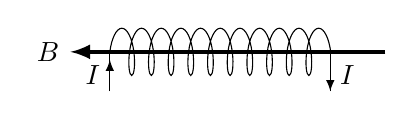
\begin{tikzpicture}
			\draw[decoration={aspect=0.3, segment length=2.5mm, amplitude=3mm,coil},decorate] (0,0) -- (3,0);
			\draw[-latex] (0,-0.5) -- (0,-0.1) node[pos=0.5, anchor=east] {\(I\)};
			\draw (0,-0.5) -- (0,0);
			\draw (2.8,-0.5) -- (2.8,0);
			\draw[-latex] (2.8,-0.1) -- (2.8,-0.5) node[pos=0.5, anchor=west] {\(I\)};
			\draw[line width=0.5mm, -latex] (3.5,0) -- (-0.5,0) node[anchor=east] {\(B\)};
		\end{tikzpicture}
	\end{center}

	\peqn{Ampere's Law for Wires}{The magnetic field strength of a current-carrying wire increases when the current is increased.}{B \propto I}
	\peqn{Ampere's Law for Solenoids}{The magnetic field strength of a current-carrying solenoid increases when the current or the number of turns is increased.}{B \propto nI}
	
	\subsection{The Motor Effect}
	\pdef{The Motor Effect}{When a current-carrying conductor is placed in a magnetic field, the conductor experiences a force. This effect on the conductor is called the motor effect.}
	The direction of the force can be determined with Fleming's left-hand rule.
	\begin{center}
		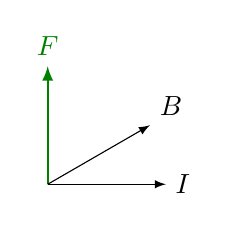
\begin{tikzpicture}
			\draw[green!50!black, thick, -latex] (0,0) -- (0,1.5) node[anchor=south] {\(\boxed{F}\)};
			\draw[-latex] (0,0) -- (1.5,0) node[anchor=west] {\(I\)};
			\draw[-latex] (0,0) -- ({1.5*sin(60)}, {1.5*cos(60)}) node[anchor=south west] {\(B\)};
		\end{tikzpicture}
		\begin{framed}
			 Le\textbf{f}t-hand rule is for induced \textbf{f}orce.
		\end{framed}
	\end{center}
	
	\subsubsection{Two Wires}
	If we have two current-carrying wires, they can either attract or repel each other.
	
	In the case of currents in the \textbf{opposite} direction, the two wires \textbf{repel} each other.
	\begin{center}
		\begin{tikzpicture}
			\draw (0,3) -- (0,0);
			\draw[-latex] (0,3) -- (0,1.5) node[pos=0.5, anchor=east] {\(I\)};
			\draw (2,3) -- (2,0);
			\draw[-latex] (2,0) -- (2,1.5) node[pos=0.5, anchor=west] {\(I\)};
			\draw[-latex] (0,1.5) -- (-0.75,1.5) node[pos=0.5, anchor=south] {\(F\)};
			\draw[-latex] (2,1.5) -- (2.75,1.5) node[pos=0.5, anchor=south] {\(F\)};
		\end{tikzpicture}
	\end{center}

	In the case of currents in the \textbf{same} direction, the two wires \textbf{attract} each other.
	\begin{center}
		\begin{tikzpicture}
			\draw (0,3) -- (0,0);
			\draw[-latex] (0,3) -- (0,1.5) node[pos=0.5, anchor=east] {\(I\)};
			\draw (2,3) -- (2,0);
			\draw[-latex] (2,3) -- (2,1.5) node[pos=0.5, anchor=west] {\(I\)};
			\draw[-latex] (0,1.5) -- (0.75,1.5) node[pos=0.5, anchor=south] {\(F\)};
			\draw[-latex] (2,1.5) -- (1.25,1.5) node[pos=0.5, anchor=south] {\(F\)};
		\end{tikzpicture}
	\end{center}
	
	These results can be derived from Fleming's left-hand rule in the examination.
	
	\subsubsection{Charges in Magnetic Fields}
	First, some notation: \(\bigodot\) means current is coming out of the paper, \(\bigotimes\) means current is going in to the paper.
	
	You should use Fleming's left-hand rule to determine where the charges would go. In the case of a positive charge, the current points \textbf{towards} where the positive charge is going; in the case of a negative charge, the current points \textbf{opposite} where the negative charge is going.
	
	\subsection{DC Motors}
	Some important parts of the DC motor:
	\begin{itemize}
		\item \textbf{Split-ring commutator:} to reverse the current every half revolution so that the motor can continue spinning.
		\item \textbf{Carbon brushes:} to ensure electrical contact between the split-ring commutator and the circuit.
	\end{itemize}

	The turning effect on a current-carrying coil in a DC motor can be increased by
	\begin{itemize}
		\item inserting a soft iron core into the coil;
		\item increasing the number of turns in the coil;
		\item increasing the current in the coil.
	\end{itemize}
\end{document}